\label{chap:diagnosis}
This chapter answers the first research question: why does a small VLM fail when it is used as a navigation agent?
It describes the benchmark's prompted agent (\cref{sec:diag-eb}), recasts its decision as a factorization that
separates perception from state (\cref{sec:diag-factor}), and then tests the three candidate causes in turn: motion
planning (\cref{sec:diag-oracle}), recognition (\cref{sec:diag-probe}), and the keeping of spatial state
(\cref{sec:diag-state}). \Cref{sec:diag-predictions} turns the diagnosis into four predictions.

\section{The prompted agent}
\label{sec:diag-eb}
The benchmark's own agent, which this thesis calls the \emph{EB prompt}, maps the image and its text history
$h_t=(u_{0:t-1},o_{0:t-1})$ directly to a plan,
\begin{equation}
(u_t,\dots,u_{t+m})=f(I_t,\ell,h_t),
\label{eq:ebpolicy}
\end{equation}
which is executed until an action fails. The prompt contains the instruction, the action list, three worked
examples, and the history, and the model must reply in a JSON format with a description of the visual state, its
reasoning, a language plan, and the action identifiers. All spatial state, namely where the target was, what the room
contains, and how the agent has turned, must be carried by $h_t$ and the generated reasoning. The thesis uses the
benchmark's prompts, examples, parser, and plan execution unchanged. With Qwen3-VL-4B, \nEBThreeParse.

\section{A factorization of the decision}
\label{sec:diag-factor}
The same decision can be factorized so that the model answers only questions about the current image and all state
lives outside it:
\begin{equation}
\begin{gathered}
(\pi_t,b_t)=f(I_t,s),\\
\mathcal{B}_t=g(\mathcal{B}_{t-1},\pi_t,b_t,D_t,p_t),\qquad u_t=\rho(\mathcal{B}_t,p_t),
\end{gathered}
\label{eq:factor}
\end{equation}
where $s$ is a target phrase, $\pi_t$ and $b_t$ are the presence probability and box of $s$ in $I_t$, the update $g$
maintains a metric belief $\mathcal{B}_t$, and the policy $\rho$ chooses the action from the belief alone.
\Cref{eq:ebpolicy,eq:factor} use the same model, the same observations, and the same actions. They differ only in
the role of the model: in \cref{eq:ebpolicy} it keeps the state and makes every decision, in \cref{eq:factor} it
answers two questions that the current image can settle. This factorization is the basis of \ours
(\cref{chap:method}) and of the controlled experiments below, which replace one part of it at a time.

\section{Planning is not the bottleneck}
\label{sec:diag-oracle}
If the factorized agent is given the true target position $x^\star$ in place of its belief about the target, with
the same occupancy map and planner, it solves \nOracle\% of the 300 test episodes: \nOracleBase\% on each of the first
four subsets and \nOracleLong\% on Long, where the agent must first turn around. The remaining failures come from the
20-step budget and from targets that cannot be approached within 1\,m. Motion planning in these rooms is therefore
nearly solved by classical geometry, and the oracle serves as the upper bound in all later comparisons.

\section{Single views are informative but unreliable}
\label{sec:diag-probe}
To measure recognition in isolation, the start view of each test episode in the first four subsets and the three
other 90$^\circ$ headings are rendered, and the VLM is queried with the target phrase $s$ on each view. A box counts
as correct if its intersection-over-union with the target's ground-truth box is at least 0.3.

Qwen3-VL-4B places a correct box on the visible target in \nProbeThreeBase, \nProbeThreeCommon, \nProbeThreeComplex,
and \nProbeThreeVisual\% of the views on Base, Common, Complex, and Visual, from 75 visible instances per subset.
Qwen2.5-VL-3B does so in \nProbeTwoBase, \nProbeTwoCommon, \nProbeTwoComplex, and \nProbeTwoVisual\%. Recognition is
therefore usable whenever the instruction names or implies a category, and weakest when it describes only appearance.

The model also errs in the other direction. On views that do not show the target, Qwen3-VL-4B still places a box in
\nFalseBoxNamedLo--\nFalseBoxNamedHi\% of the cases for named categories and in \nFalseBoxVisual\% for appearance-only
phrases. \Cref{tab:probe,fig:probe} give both rates for both models. The two models make different trade-offs.
Qwen3-VL-4B finds the target about twice as often as Qwen2.5-VL-3B, but it also places more boxes on views that do
not show the target, most of all for appearance-only phrases. Qwen2.5-VL-3B answers more conservatively and misses
more targets. Neither model is reliable enough to act on one answer: the first would follow look-alikes, the second
would walk past targets. A single answer is therefore evidence, not a decision.

\begin{figure}[htbp]
\centering
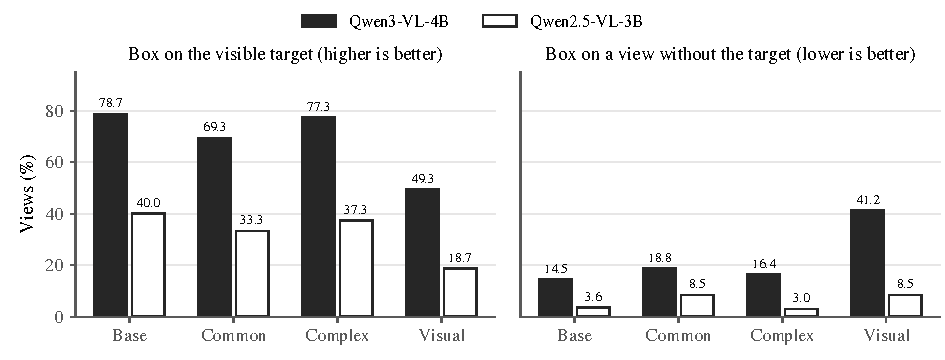
\includegraphics[width=\linewidth]{figures/th_probe.pdf}
\caption[Recognition from single views]{Recognition from single views (\cref{tab:probe}). Left: views showing the
target in which the model places a box with IoU${\ge}0.3$ on it. Right: views without the target in which the model
still places a box.}
\label{fig:probe}
\end{figure}
An agent that acts on every box would be drawn to look-alikes; an agent that ignores weak boxes would miss real
targets. This observation motivates the evidence accumulation of \cref{sec:method-memory}.

\begin{table}[htbp]
\centering\small
\caption[Single-view probe]{Single-view probe on the test episodes of the first four subsets (start view and the
three other 90$^\circ$ headings; 75 views with the target visible per subset).}
\label{tab:probe}
\begin{tabular*}{\linewidth}{@{\extracolsep{\fill}}lcccccccc@{}}
\toprule
& \multicolumn{4}{c}{Box on the target, IoU${\ge}0.3$ (\%)} & \multicolumn{4}{c}{Box on a view without it (\%)}\\
\cmidrule(lr){2-5}\cmidrule(l){6-9}
Model & Base & Common & Complex & Visual & Base & Common & Complex & Visual\\
\midrule
Qwen3-VL-4B & 78.7 & 69.3 & 77.3 & 49.3 & 14.5 & 18.8 & 16.4 & 41.2\\
Qwen2.5-VL-3B & 40.0 & 33.3 & 37.3 & 18.7 & 3.6 & 8.5 & 3.0 & 8.5\\
\bottomrule
\end{tabular*}

\end{table}

\section{The prompted agent loses spatial state}
\label{sec:diag-state}
If neither planning nor recognition explains the failure, the remaining candidate is the keeping of spatial state.
The failure taxonomy of \cref{sec:pre-metrics} tests this directly. Of the \nFailEBThree{} episodes that the EB prompt
fails with Qwen3-VL-4B, \nLostEBThree{} lose a target that was in view, \nBlockedEBThree{} are blocked by collisions,
and \nNearEBThree{} end within 1.5\,m of the target. In \nNeverLongEBThree{} Long episodes the agent never brings the
target into view at all.

The same pattern holds for the smaller model. With Qwen2.5-VL-3B the EB prompt loses a target it has seen in
\nLostEBTwo{} of the 300 episodes, more than with Qwen3-VL-4B, which shows that the problem grows as the model shrinks
(\cref{tab:taxonomy}).

Each of these failure modes is a failure of state. A target that was in view and is lost shows that the agent did not
remember where it was. Repeated collisions show that the agent did not remember which moves were rejected or where
the furniture is. A target behind the agent that is never seen shows that the agent did not keep track of which
directions it had already looked in. In every case the information was available to the agent at some step, and
in every case it had to be carried forward as generated text, which the model neither verifies against the image
nor updates consistently.

\subsection{An episode in detail}
\Cref{tab:eb-excerpt} follows the EB prompt with Qwen3-VL-4B through the first plans of one Long-horizon test
episode, in which the target is a pot and the agent starts facing away from it. At the first two steps the model
writes that the pot is on the counter to its right, although the simulator shows that the pot is not in view. It
plans moves toward this imagined pot, the moves run into the counter, and the model keeps planning the same moves.
Over the episode \tExcerptRejected{} of \tExcerptSteps{} actions are rejected and the pot is \tExcerptSeen{} seen. With
the same model on the same episode, \ours turns, finds the pot, and \tExcerptSOk{} in \tExcerptSSteps{} steps.

\begin{table}[htbp]
\centering\small
\caption[The EB prompt on one Long-horizon episode]{The first four plans of the EB prompt (Qwen3-VL-4B) on a
Long-horizon test episode whose target is a pot. ``Target in view'' comes from the simulator and is not available to
the agent; the last column counts the accepted and rejected actions of each plan.}
\label{tab:eb-excerpt}
\begin{tabular}{@{}rp{0.42\linewidth}cp{0.17\linewidth}c@{}}
\toprule
Step & Model's description of the view & In view & Plan & Acc./rej.\\
\midrule
0 & \textit{``The Pot is located on the countertop to the right side of the kitchen, near the stove.''} & no & right & 1 / 0\\
1 & \textit{``The Pot is located on the countertop to the right side of the kitchen, near the stove.''} & no & forward, forward, forward & 2 / 1\\
4 & \textit{``The current view shows a kitchen area with wooden cabinets on both sides.''} & no & right, forward, forward & 0 / 1\\
5 & \textit{``The current view shows a kitchen area with wooden cabinets on both sides.''} & no & right, forward, forward & 0 / 1\\
\bottomrule
\end{tabular}

\end{table}

The excerpt shows the mechanism of the failure. The model's description of the view is a belief, not an observation,
and nothing in the agent compares this belief with the image. Once written, the belief is carried into the next
prompt as part of the history and shapes the next plan. The rejected moves are recorded in the history as well, but
the model does not connect them with a wrong belief about where the target is.

\subsection{Why text is a poor carrier of spatial state}
Three properties of generated text explain why a small model cannot use it to keep spatial state.
\begin{enumerate}
\item \textbf{No grounding.} A sentence such as ``the pot is to my right'' has no coordinates. After the agent
turns, the sentence is no longer true, and the model must rewrite it from memory of the turn.
\item \textbf{No accumulation.} Text records one belief at a time. It has no natural way to express that a location
was confirmed from three viewpoints and contradicted from one, so evidence does not add up.
\item \textbf{No check.} The model generates the next belief conditioned on its previous one. A wrong belief is
therefore more likely to be repeated than corrected, as in \cref{tab:eb-excerpt}.
\end{enumerate}
A metric representation has the opposite properties: a position stays valid when the agent turns, evidence can be
added and subtracted, and every new frame can be compared with every stored hypothesis.

\section{Four testable predictions}
\label{sec:diag-predictions}
The diagnosis can be wrong, so it is stated as predictions that the experiments of \cref{chap:experiments} can
falsify. If small VLMs fail because their role makes them carry spatial state through text, an agent that keeps this
state outside the model, with the same model and the same actions, should
\begin{enumerate}[label=(\roman*)]
\item remove the never-seen and blocked failures and reduce the lost-after-seen ones;
\item gain most on Long, where the target must be remembered across turns;
\item gain least on Visual, where single-view recognition is weakest and remains the limit; and
\item depend far less on the size of the model, which no longer plans.
\end{enumerate}

\section{Summary}
\Cref{tab:diagnosis-summary} summarizes the diagnosis. Planning and recognition are adequate for the task; the
keeping of spatial state is not. The next chapter builds an agent that removes this burden from the model.

\begin{table}[htbp]
\centering\small
\caption{Summary of the diagnosis with Qwen3-VL-4B on the EB-Navigation test set.}
\label{tab:diagnosis-summary}
\begin{tabular}{@{}p{0.27\linewidth}p{0.36\linewidth}p{0.29\linewidth}@{}}
\toprule
Candidate cause & Evidence & Verdict\\
\midrule
Motion planning & oracle target: \nOracle\% success & not the bottleneck\\
Recognition & correct box on \nProbeThreeCommon--\nProbeThreeBase\% of visible named targets; false boxes on
\nFalseBoxNamedLo--\nFalseBoxNamedHi\% of empty views & usable, but unreliable alone\\
Spatial state & \nLostEBThree{} lost after seen, \nBlockedEBThree{} blocked, \nNeverLongEBThree{} Long never seen &
the bottleneck\\
\bottomrule
\end{tabular}
\end{table}
